\section{Sharpness on a fixed cube}
\label{sec:sharpness}

We first prove that the exponent in \Cref{main:stability} cannot be
improved. The example uses three affine functions, with a small change
in one slope reassigning source points between the central and outer
cells. The following observation identifies the resulting gradients as
optimal maps. It applies to the general source body $K$ of the introduction.

\begin{lemma}[Optimality of a finite affine maximum]
\label{cells:optimality}
Let
\[
 u(x)=\max_{1\le i\le N}\bigl(x\cdot y_i+c_i\bigr).
\]
For $\rho$-almost every $x$, all maximizing indices have the same slope.
Define $T(x)=y_i$ for the smallest maximizing index $i$, and put
$\lambda=T_\#\rho$. Then $T$ is Borel, $T=\nabla u$ almost everywhere, and
the transport plan $(\id,T)_\#\rho$ is the unique quadratic-cost optimal
plan from $\rho$ to $\lambda$.
\end{lemma}

\begin{proof}
The first-index choice is Borel because its level sets are given by
finitely many strict and non-strict affine inequalities.
Merge repeated slopes, retaining the largest intercept for each slope, and
write the resulting intercept as $c(y)$. Ties between distinct slopes lie
in a finite union of hyperplanes. Outside this null set, the maximizing
affine function remains strictly maximal in a neighborhood, so its slope
is the gradient of $u$.

For every transport plan $\pi$ from $\rho$ to $\lambda$, the inequality
$x\cdot y+c(y)\le u(x)$ gives
\[
 \int x\cdot y\,d\pi(x,y)
 \le \int_K u\,d\rho-\int c(y)\,d\lambda(y).
\]
The graph plan of $T$ attains equality. Since the two marginals fix the
integrals of $|x|^2$ and $|y|^2$, maximizing the displayed scalar product is
equivalent to minimizing quadratic cost. Equality for any optimal plan
requires it to be concentrated on pairs $(x,y)$ with
$x\cdot y+c(y)=u(x)$. The maximizing slope is unique for $\rho$-almost every
$x$, so the plan is concentrated on the graph of $T$. This proves
uniqueness of the plan.
\end{proof}

We now specialize to the cube. The two targets below have the same atom
masses, but their optimal maps differ on a much larger part of the source
than their target displacement alone might suggest.

\begin{proposition}[Optimality of the exponent]\label{sharpness:exponent}
For every fixed $d\ge2$, let $K=Y=[-1,1]^d$ and
$\rho=2^{-d}1_K\,dx$.  For every $\alpha>1/3$,
\[
 \sup_{\substack{\mu,\nu\in\Prob(Y)\\ \mu\ne\nu}}
 \frac{\|T_\mu-T_\nu\|_{L^2(\rho)}}{W_2(\mu,\nu)^\alpha}
 =+\infty.
\]
The supremum remains infinite when both targets are required to have
exactly three atoms.
\end{proposition}

\begin{proof}
For $0<a<1/2$, put $b=a/2$ and define
\begin{equation}\label{sharpness:potentials}
 u_a(x)=\max\{-x_1,x_1,a\},\qquad
 \widetilde u_a(x)=\max\{-x_1,x_1,a+bx_2\}.
\end{equation}
Let $\mu_a=(\nabla u_a)_\#\rho$ and
$\nu_a=(\nabla\widetilde u_a)_\#\rho$, with any fixed first-index
selection on the null tie sets.  Their slopes are, respectively,
$-e_1,e_1,0$ and $-e_1,e_1,be_2$, all in the fixed set $Y$.
By \Cref{cells:optimality}, these gradients are the unique optimal
maps to their laws.

Since $a/2\le a+bx_2\le3a/2<1$, the central cells are, up to null
boundaries,
\[
 A_a=\{x\in K:|x_1|<a\},\qquad
 B_a=\{x\in K:|x_1|<a+bx_2\}.
\]
Tilting the central strip preserves its mass but changes which points
receive a central or an outer slope. \Cref{fig:sharpness-cells} shows
the symmetric difference where this reassignment occurs.

\begin{figure}[tbp]
\centering
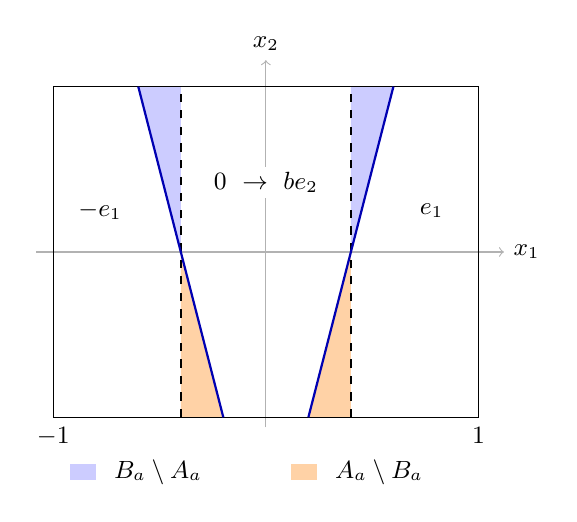
\begin{tikzpicture}[x=2.7cm,y=2.1cm,font=\small]
 \fill[blue!20] (-0.4,0)--(-0.6,1)--(-0.4,1)--cycle;
 \fill[blue!20] (0.4,0)--(0.6,1)--(0.4,1)--cycle;
 \fill[orange!35] (-0.4,0)--(-0.4,-1)--(-0.2,-1)--cycle;
 \fill[orange!35] (0.4,0)--(0.4,-1)--(0.2,-1)--cycle;
 \draw[gray!60,->] (-1.08,0)--(1.12,0) node[right,text=black] {$x_1$};
 \draw[gray!60,->] (0,-1.06)--(0,1.16) node[above,text=black] {$x_2$};
 \draw (-1,-1) rectangle (1,1);
 \draw[dashed,thick] (-0.4,-1)--(-0.4,1);
 \draw[dashed,thick] (0.4,-1)--(0.4,1);
 \draw[blue!70!black,thick] (-0.2,-1)--(-0.6,1);
 \draw[blue!70!black,thick] (0.2,-1)--(0.6,1);
 \node[fill=white,inner sep=2pt] at (-0.78,0.25) {$-e_1$};
 \node[fill=white,inner sep=2pt] at (0.78,0.25) {$e_1$};
 \node[fill=white,inner sep=2pt] at (0,0.42) {$0\ \to\ be_2$};
 \node[below] at (-1,-1) {$-1$};
 \node[below] at (1,-1) {$1$};
 \fill[blue!20] (-0.92,-1.38) rectangle (-0.8,-1.28);
 \node[right] at (-0.76,-1.33) {$B_a\setminus A_a$};
 \fill[orange!35] (0.12,-1.38) rectangle (0.24,-1.28);
 \node[right] at (0.28,-1.33) {$A_a\setminus B_a$};
\end{tikzpicture}
\caption{A source-coordinate section of the cube example, drawn with
$a=2/5$ and $b=a/2$. Dashed lines bound $A_a$; solid blue lines bound
$B_a$. The two shaded sets have equal area, so the central mass stays
fixed. On their union, source points switch between central and outer
slopes. The labels show map values on the unchanged outer regions and
the common central region; they are not target points plotted in the
source plane. The remaining coordinates integrate out.}
\label{fig:sharpness-cells}
\end{figure}

On $A_a$, the first map is zero; on its complement it is
$\operatorname{sign}(x_1)e_1$.  The second map equals $be_2$ on
$B_a$ and $\operatorname{sign}(x_1)e_1$ on its complement.
Under $\rho$, the coordinates are independent and uniform on
$[-1,1]$.  On the slice $x_2=t$, the second central interval has
probability $a+bt$, and each outer interval has probability
$(1-a-bt)/2$.  Averaging over $t$ gives
\begin{equation}\label{sharpness:targets}
 \mu_a=\frac{1-a}{2}(\delta_{-e_1}+\delta_{e_1})+a\delta_0,
 \qquad
 \nu_a=\frac{1-a}{2}(\delta_{-e_1}+\delta_{e_1})+a\delta_{be_2}.
\end{equation}
Both targets have three distinct atoms of positive mass.

The coupling that fixes the outer atoms and moves the central atom
from $0$ to $be_2$ has squared cost $ab^2$.  Conversely, every point
in the support of $\mu_a$ has second coordinate zero.  Every coupling
$\pi$ of the two targets therefore satisfies
\[
 \int|y-z|^2\,d\pi(y,z)
 \ge\int|y_2-z_2|^2\,d\pi(y,z)=ab^2.
\]
Consequently,
\begin{equation}\label{sharpness:target-distance}
 W_2(\mu_a,\nu_a)^2=ab^2.
\end{equation}
The same matching coupling costs $ab$ for $W_1$, while every coupling
has cost at least
$\int|y_2-z_2|\,d\pi=ab$. Thus
\begin{equation}\label{sharpness:w1-distance}
 W_1(\mu_a,\nu_a)=ab=\frac{a^2}{2}.
\end{equation}

The two central intervals on the slice $x_2=t$ are nested, and their
symmetric difference has conditional probability $b|t|$.  Thus
\[
 \rho(A_a\mathbin{\triangle}B_a)
 =\frac12\int_{-1}^1b|t|\,dt=\frac b2.
\]
The first coordinate of the map difference contributes the indicator
of that symmetric difference, and its second coordinate contributes
$b^2$ on $B_a$.  Orthogonality gives the pointwise identity
\[
 |T_{\mu_a}-T_{\nu_a}|^2
 =1_{A_a\mathbin{\triangle}B_a}+b^2 1_{B_a}
 \quad\rho\hbox{-almost everywhere}.
\]
Since $\rho(B_a)=a$, this proves
\begin{equation}\label{sharpness:map-distance}
 \|T_{\mu_a}-T_{\nu_a}\|_{L^2(\rho)}^2=\frac b2+ab^2.
\end{equation}
The remaining $d-2$ coordinates integrate out, so all computations
hold in every fixed dimension $d\ge2$.

Substituting $b=a/2$ into \eqref{sharpness:target-distance} and
\eqref{sharpness:map-distance} gives
\[
 W_2(\mu_a,\nu_a)=\frac{a^{3/2}}2,
 \qquad
 \|T_{\mu_a}-T_{\nu_a}\|_{L^2(\rho)}
 =\frac{\sqrt a}{2}\sqrt{1+a^2}.
\]
For every $\alpha>1/3$, their ratio is
\[
 \frac{\|T_{\mu_a}-T_{\nu_a}\|_{L^2(\rho)}}
      {W_2(\mu_a,\nu_a)^\alpha}
 =2^{\alpha-1}\sqrt{1+a^2}\,a^{(1-3\alpha)/2}
 \longrightarrow+\infty\qquad(a\downarrow0).
\]
The source, target container, and number of atoms stay fixed,
proving the proposition.
\end{proof}
